\chapter{Introduction}

In this robotics class, we consider the task of making a person hold his/her Raspberry Pi in front of a laptop's webcam.  The Raspberry Pi, equipped with its sense hat,  allows to display a single red dot on its LED matrix so that the webcam can monitor it. The goal of this project is to ensure that the red dot always remains as close as possible to the webcam's captured image. This must particularly hold if the person shakes, moves, or rotates the Raspberry Pi in front of the webcam. If the Raspberry Pi's LED matrix is placed too far from the webcam's image center, the red dot should be placed as close as possible to the latter.

If we were to solve this problem manually, we would need to have access to the Raspberry Pi's accelerometer and gyroscope to determine the speed and the direction of the motion of the red dot on the LED matrix. This would require us to use a reference frame for which the origin would be the center of the webcam's image. Access to acceleration and gyroscopic data would allow to construct a velocity vector anchored at the red dot and pointing towards the origin of this reference frame. Doing so would enable us to undo the person's motions and therefore stabilize the red dot at the center of the image. Although this approach seems technically feasible, its implementation is not straightforward. 

In this course, we intend to use Reinforcement Learning (RL) as a "last-resort" solution to overcome the complexity of the previous approach. Our goal is thus to produce a \textit{policy} that allows to move the red dot on the Raspberry Pi's LED matrix so as to be as close as possible to the center of the image. In order to achieve this goal, we will need the following components:

\begin{itemize}
	\item A Raspberry Pi with a mounted sense hat (comprises the LED matrix);
	\item A laptop with a front webcam;
	\item A Reinforcement Learning agent.
\end{itemize}

In the following sections, we start by explaining how the Raspberry Pi can be set up to communicate with the laptop about the red dot's position on the webcam image.  We also describe how the red dot's position can be retrieved from the raw image using image processing techniques. The last section of this chapter investigates the set up of the RL agent and its corresponding environment.

\section{Configuration of the Raspberry Pi}

In order for the RL agent to decide how to move the red dot on the Raspberry Pi 's LED matrix, the agent must have access to acceleration and gyroscopic data of the Pi. In return, the Pi must have access to the decision of the agent, given this data, in order to re-center the red dot. The actions of the agent are (1) \textit{Move North}, (2) \textit{Move South}, (3) \textit{Move West}, (4) \textit{Move East} and (5) \textit{Stay}.  Both entities thus communicate according to the scheme of figure \ref{communication}.

\begin{figure}

\centering

\begin{tikzpicture}[
squarednode/.style={rectangle, draw=black!60, fill=black!5, very thick, minimum size=5mm},
]
%Nodes
\node[squarednode]      (agent)                             {RL Agent};
\node[squarednode]      (rasp)   [right=of agent] {Raspberry Pi};

%Lines
\draw[->] (agent.north) to [out=90,in=90]     node[midway,  above]   {Action: North, South, West, East, Stay}  (rasp.north) ;
\draw[->] (rasp.south)   to [out=-90,in=-90]  node[midway, below]    {Acceleration $\&$ Gyroscope}             (agent.south);

\end{tikzpicture}

\caption{Communication between the Raspberry Pi and the RL agent. The Pi sends its acceleration and gyroscopic data over to the agent which decides what action to take in order to re-center the red dot on the Pi.} 
\label{communication}
\end{figure}

To ensure a communication between both entities, we implement a Python socket server on the on both sides over the same wifi network. On the Pi, we create a python socket server using code inspired from the project description. Section \ref{server_code} of the Appendix illustrates this process. Apart from the functions for sending and receiving objects from/to the server, a Sensehat instance is created, along with a Raspberry instance. The Sensehat object is responsible for

\begin{enumerate}
\item displaying the LED light through its \texttt{\detokenize{set_pixel()}} method;
\item sampling acceleration data through its  \texttt{\detokenize{get_accelerometer_raw()}} method;
\item sampling gyroscopic data through its  \texttt{\detokenize{get_gyroscope_raw()}} method.
\end{enumerate}

The Raspberry instance on the other hand wraps the Sensehat instance into a class which has these acceleration and orientation measures as properties.  The code of section \ref{rasp_code} illustrates this process. In order to close the loop of figure \ref{communication}, the Raspberry instance needs a function that translates the action prescribed by the agent into a visible result. This is exactly the purpose of the  \texttt{\detokenize{move_led()}} function of this class, which executes all five actions described above.

\section{Webcam image processing}

For the agent to prescribe actions to the Pi as shown on figure \ref{communication}, it must be able to detect the position of the red dot on the LED matrix. It is clear that the reliable nature of the detection of this red dot is crucial for the project's success. Indeed, if this detection were to fail or to produce imprecise results, it would inevitably affect the learning of the agent. For our agent to learn properly, it is crucial to develop a technique that extracts the position of the red dot from the webcam's image with small influence of the surrounding light. We will use the OpenCV library to perform this task. A first step toward this task is to get familiar with standard image processing techniques proposed by OpenCV. One important feature is the use of \textit{masks} to process an image. Such masks basically filter out specific regions of an HSV image so as to produce an image with enhanced contrasts for certain objects. In our case, we wish to extract the regions of the image with bright red colours. An important drawback of the Pi's LED matrix is that the red light seen by us humans is, in fact, not predominantly red. The emitted light is indeed shifted towards ultraviolet wavelengths, which makes its detection hard, especially in when placed in an environment with daily light as the one of figure \ref{no_filter}. Thus before implementing a complete filtering of the image's red components, I decided to get a feeling of how the filtered image reacts to cuts in \textit{h}, \textit{s} and \textit{v} values. I therefore used the script of section \ref{calibrate} to produce cursors that filter the image in real time. Figure \ref{filter} shows the result of applying $h \in [0, 45] $,  $s \in [0, 255]$ and $v \in [150, 255]$. After playing around with those cursors, I came up with the following conclusions:

\begin{itemize}
	\item The image is very sensitive to  \texttt{\detokenize{s_min}} (keep it at $0$);
	\item Proper red filtering can only be done using two intervals of \texttt{\detokenize{h}} around $0$ and $180$;
	\item Only very high brightness allows to discriminate daily light from the Pi's LED light (keep \texttt{\detokenize{v}} between $217$ and $255$)
\end{itemize}

\begin{figure}[H]

  \begin{minipage}[b]{0.45\linewidth}
   \centering
   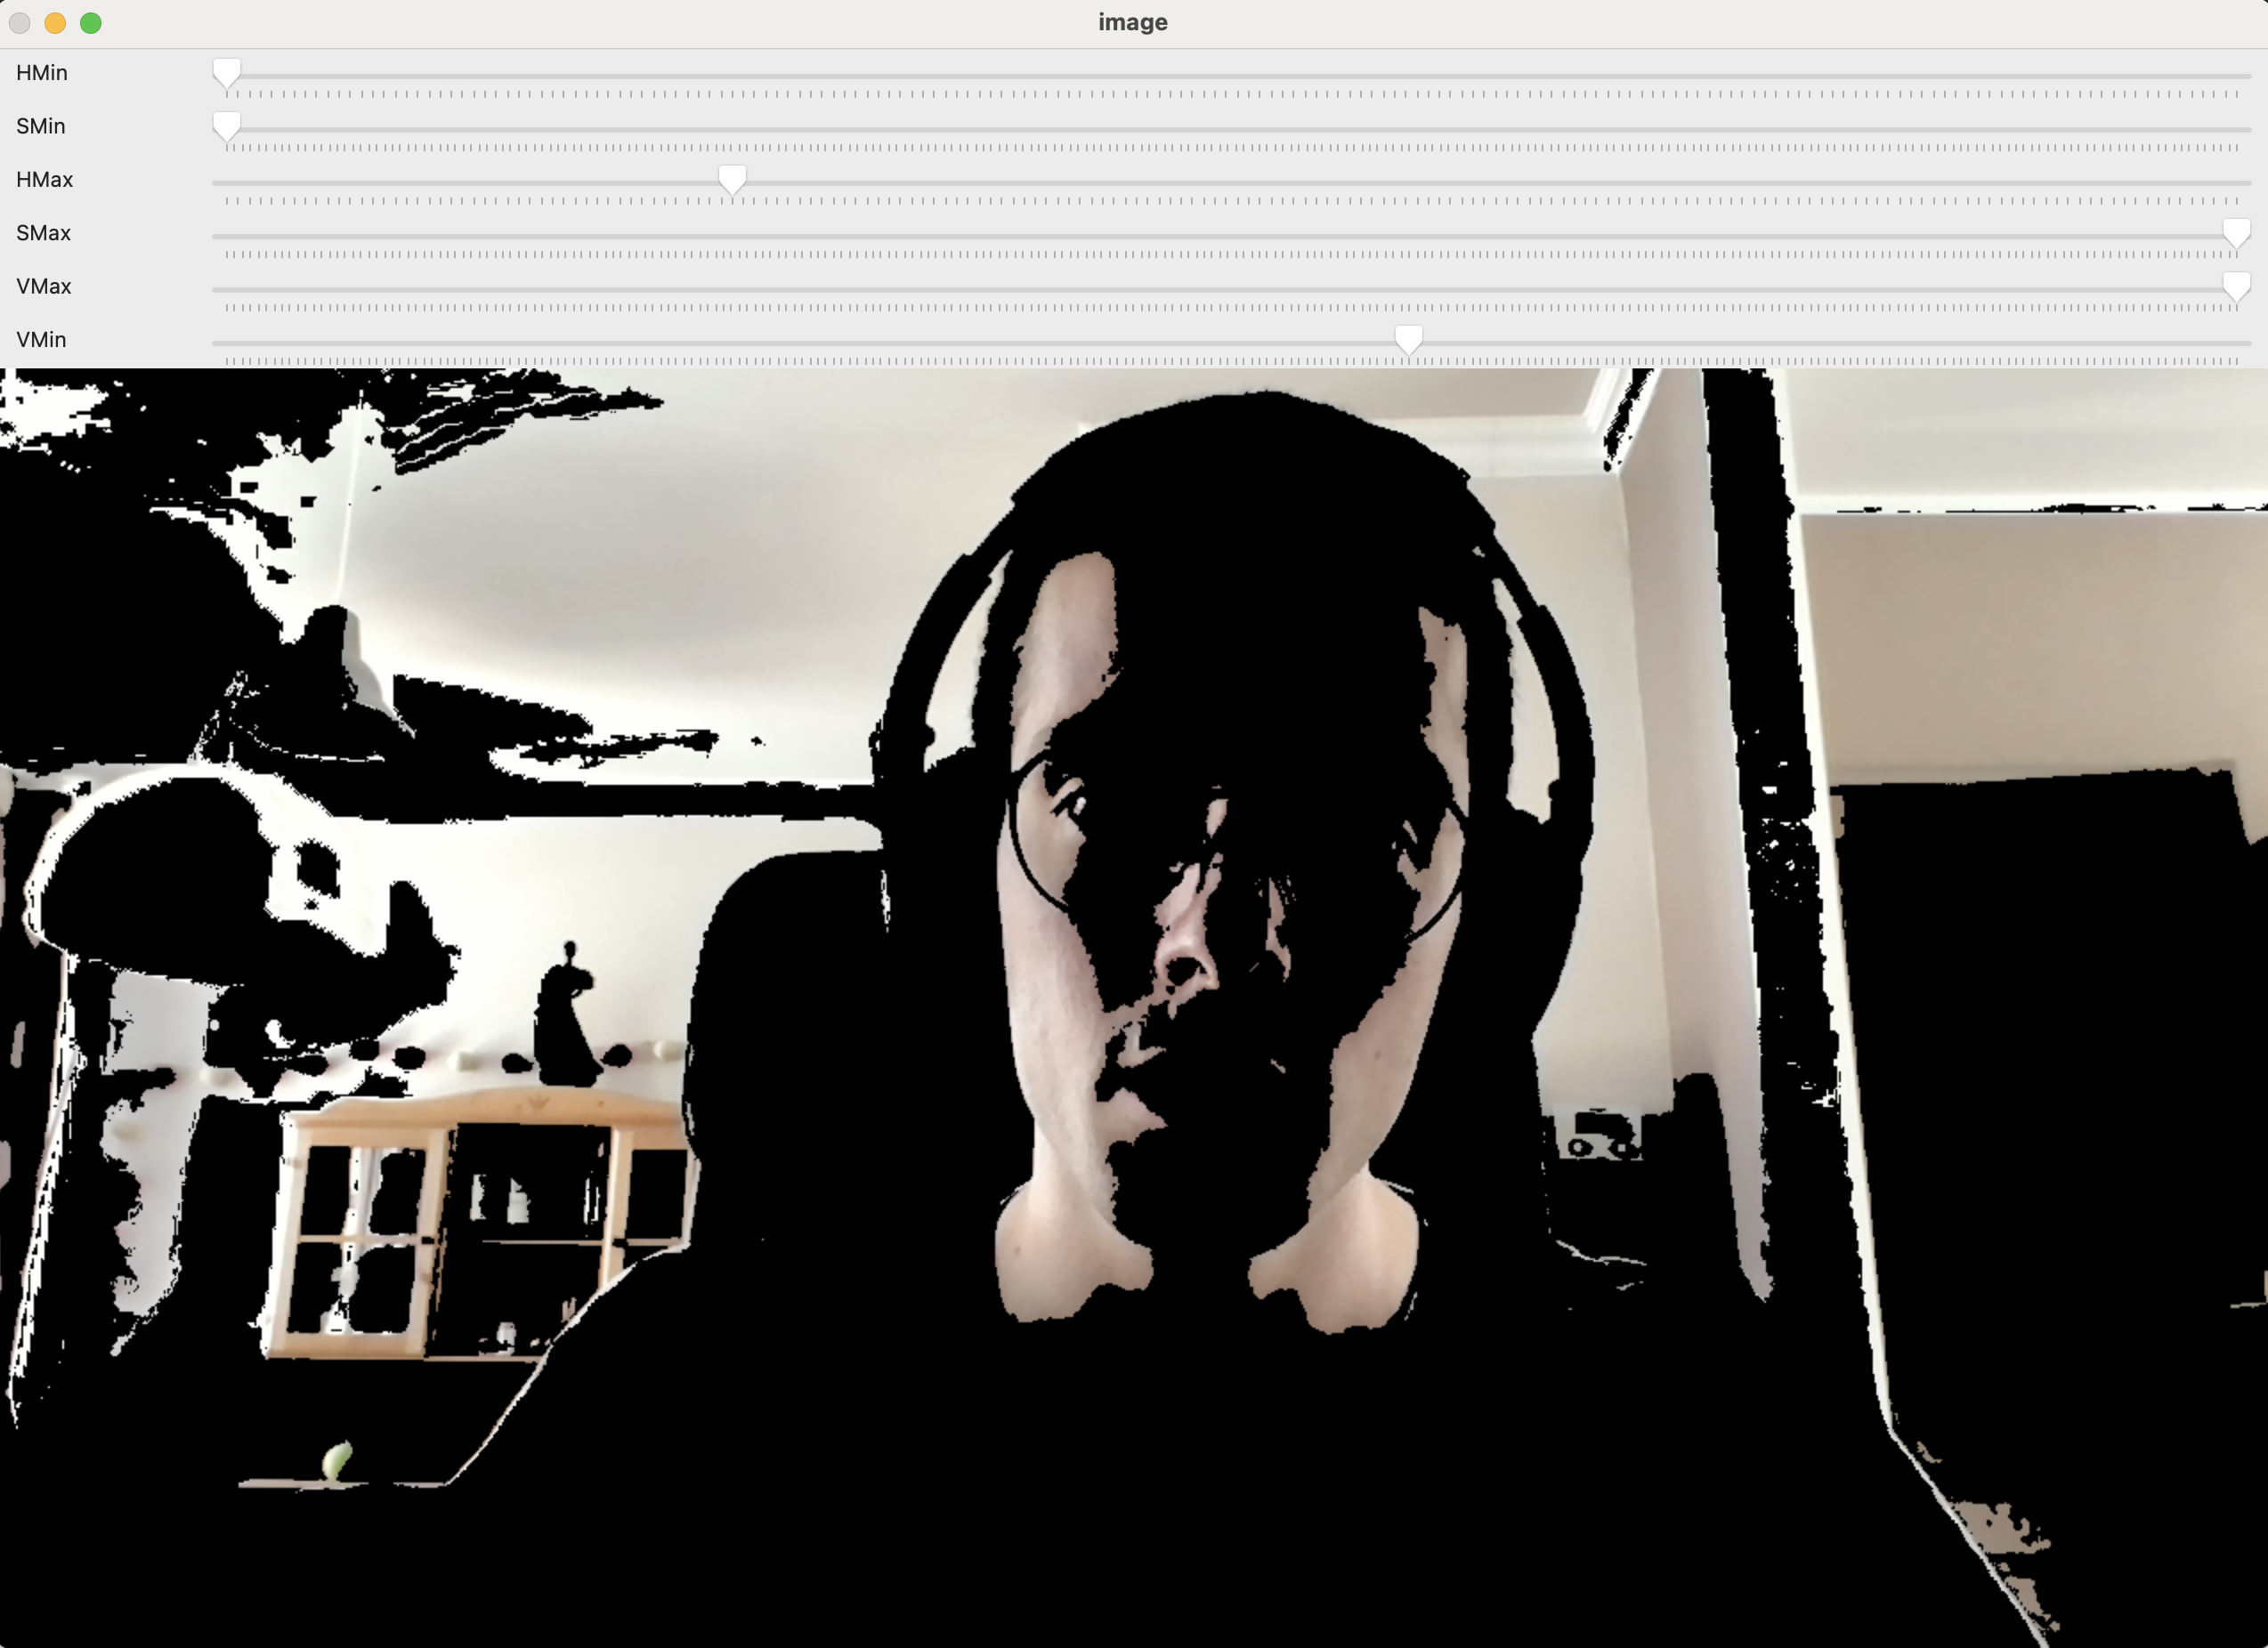
\includegraphics[width=6.5cm,height=5cm]{Images/calibrate.png}
   \caption{Image processing using OpenCV with $h \in [0, 45] $,  $s \in [0, 255]$ and $v \in [150, 255]$.}
   \label{filter}
  \end{minipage}
\hfill
  \begin{minipage}[b]{0.45\linewidth}
   \centering
   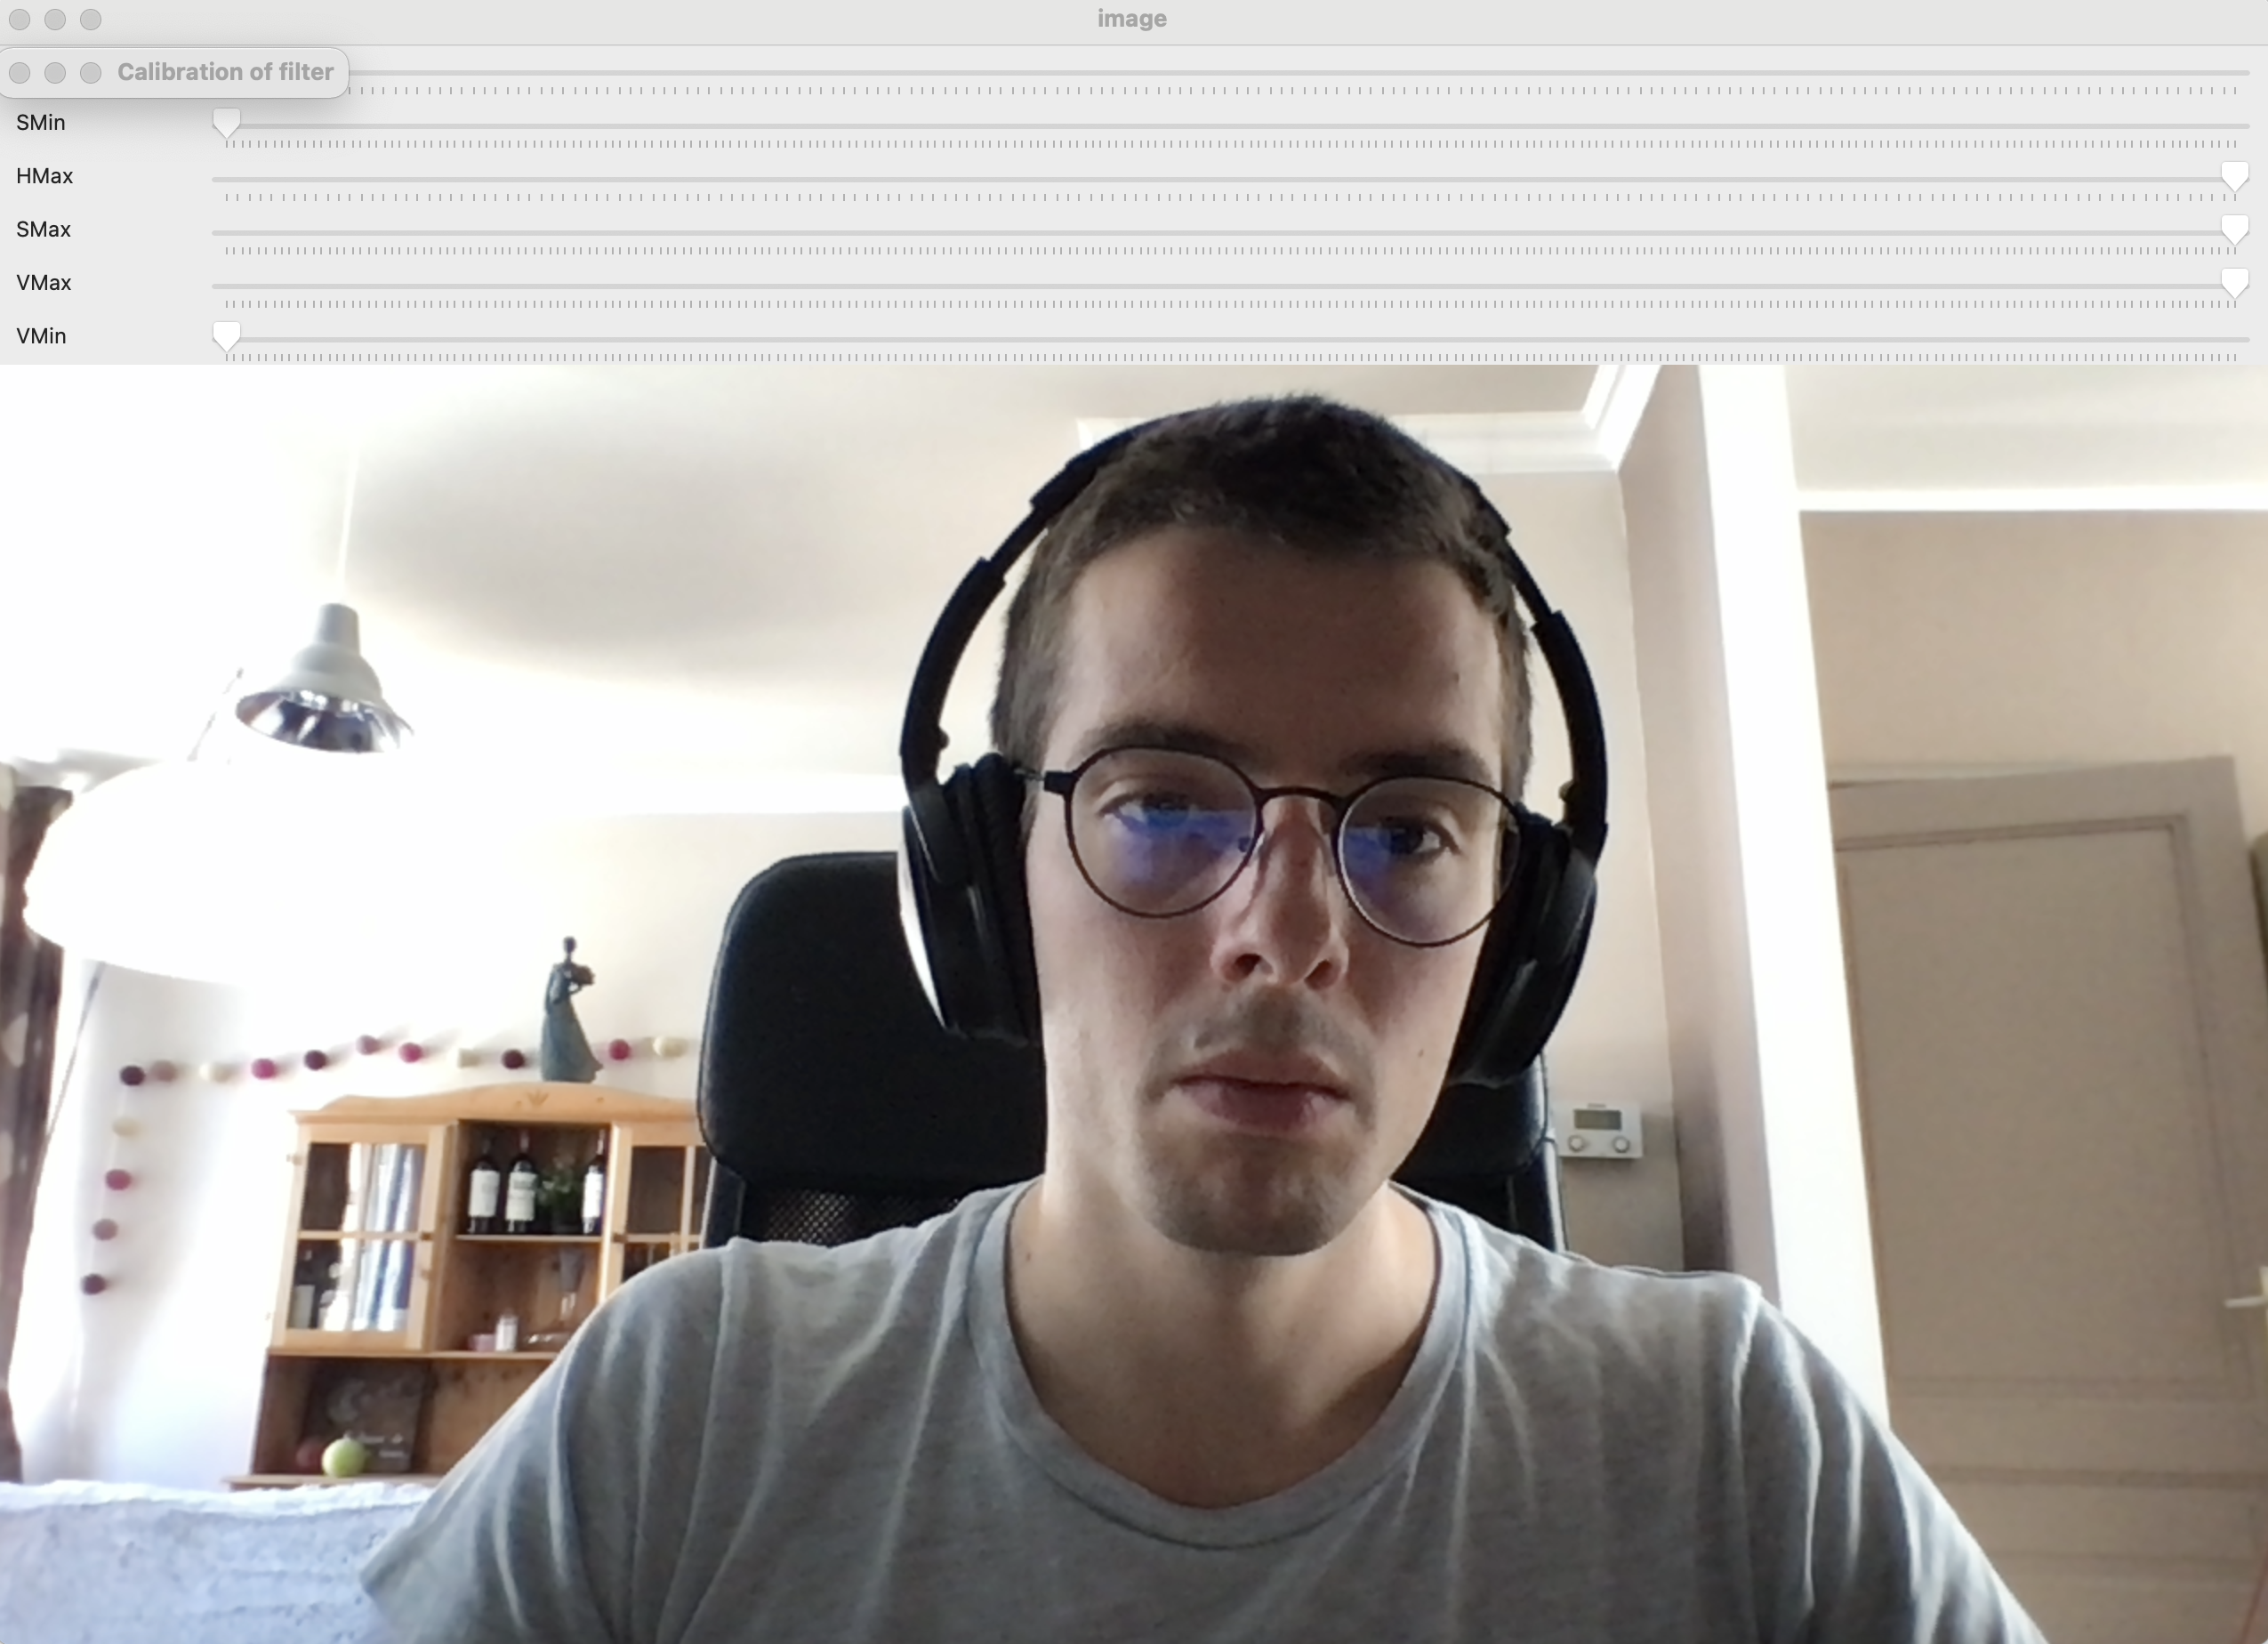
\includegraphics[width=6.5cm,height=5cm]{Images/calibrate2.png}
   \caption{Original image with no filter.}
   \label{no_filter}
  \end{minipage}
\end{figure}

This first trial with the OpenCV library helped me produce a full preprocessing pipeline of the original webcam image. The function \texttt{\detokenize{filter_image()}} of section \ref{processing} implements this process:

\begin{enumerate}
	\item Apply a first lower and upper mask using $h \in [0, 10] \cup [90,179] $,  $s \in [0, 255] \cup [0,255]$ and $v \in [217, 255] \cup [230,255]$;
	\item Re-apply a red filter using $h \in [10, 180] $,  $s \in [0, 150]$ and $v \in [0, 255]$;
	\item Filter the image using a binary threshold set on $150$ pixel value.
\end{enumerate}

The careful reader will however have noticed that the red dot itself was not captured by these processing techniques. Instead the \textit{contour} of the LED cell was highlighted (see final figure \ref{opencv:threshold}). The idea of capturing the contour of the dot rather than its center was forced by the fact that the LED light seemed to somehow "burn" the built-in camera of my Macbook, making its center invisible after applying the first red filter.  In addition, applying the \texttt{\detokenize{compute_red_dot()}} function of section \ref{processing} allows to get back our red dot since OpenCV's \texttt{\detokenize{connectedComponentsWithStats()}} function computes the position of the biggest visible area. 

\begin{figure}[H]

  \begin{minipage}[b]{0.45\linewidth}
   \centering
   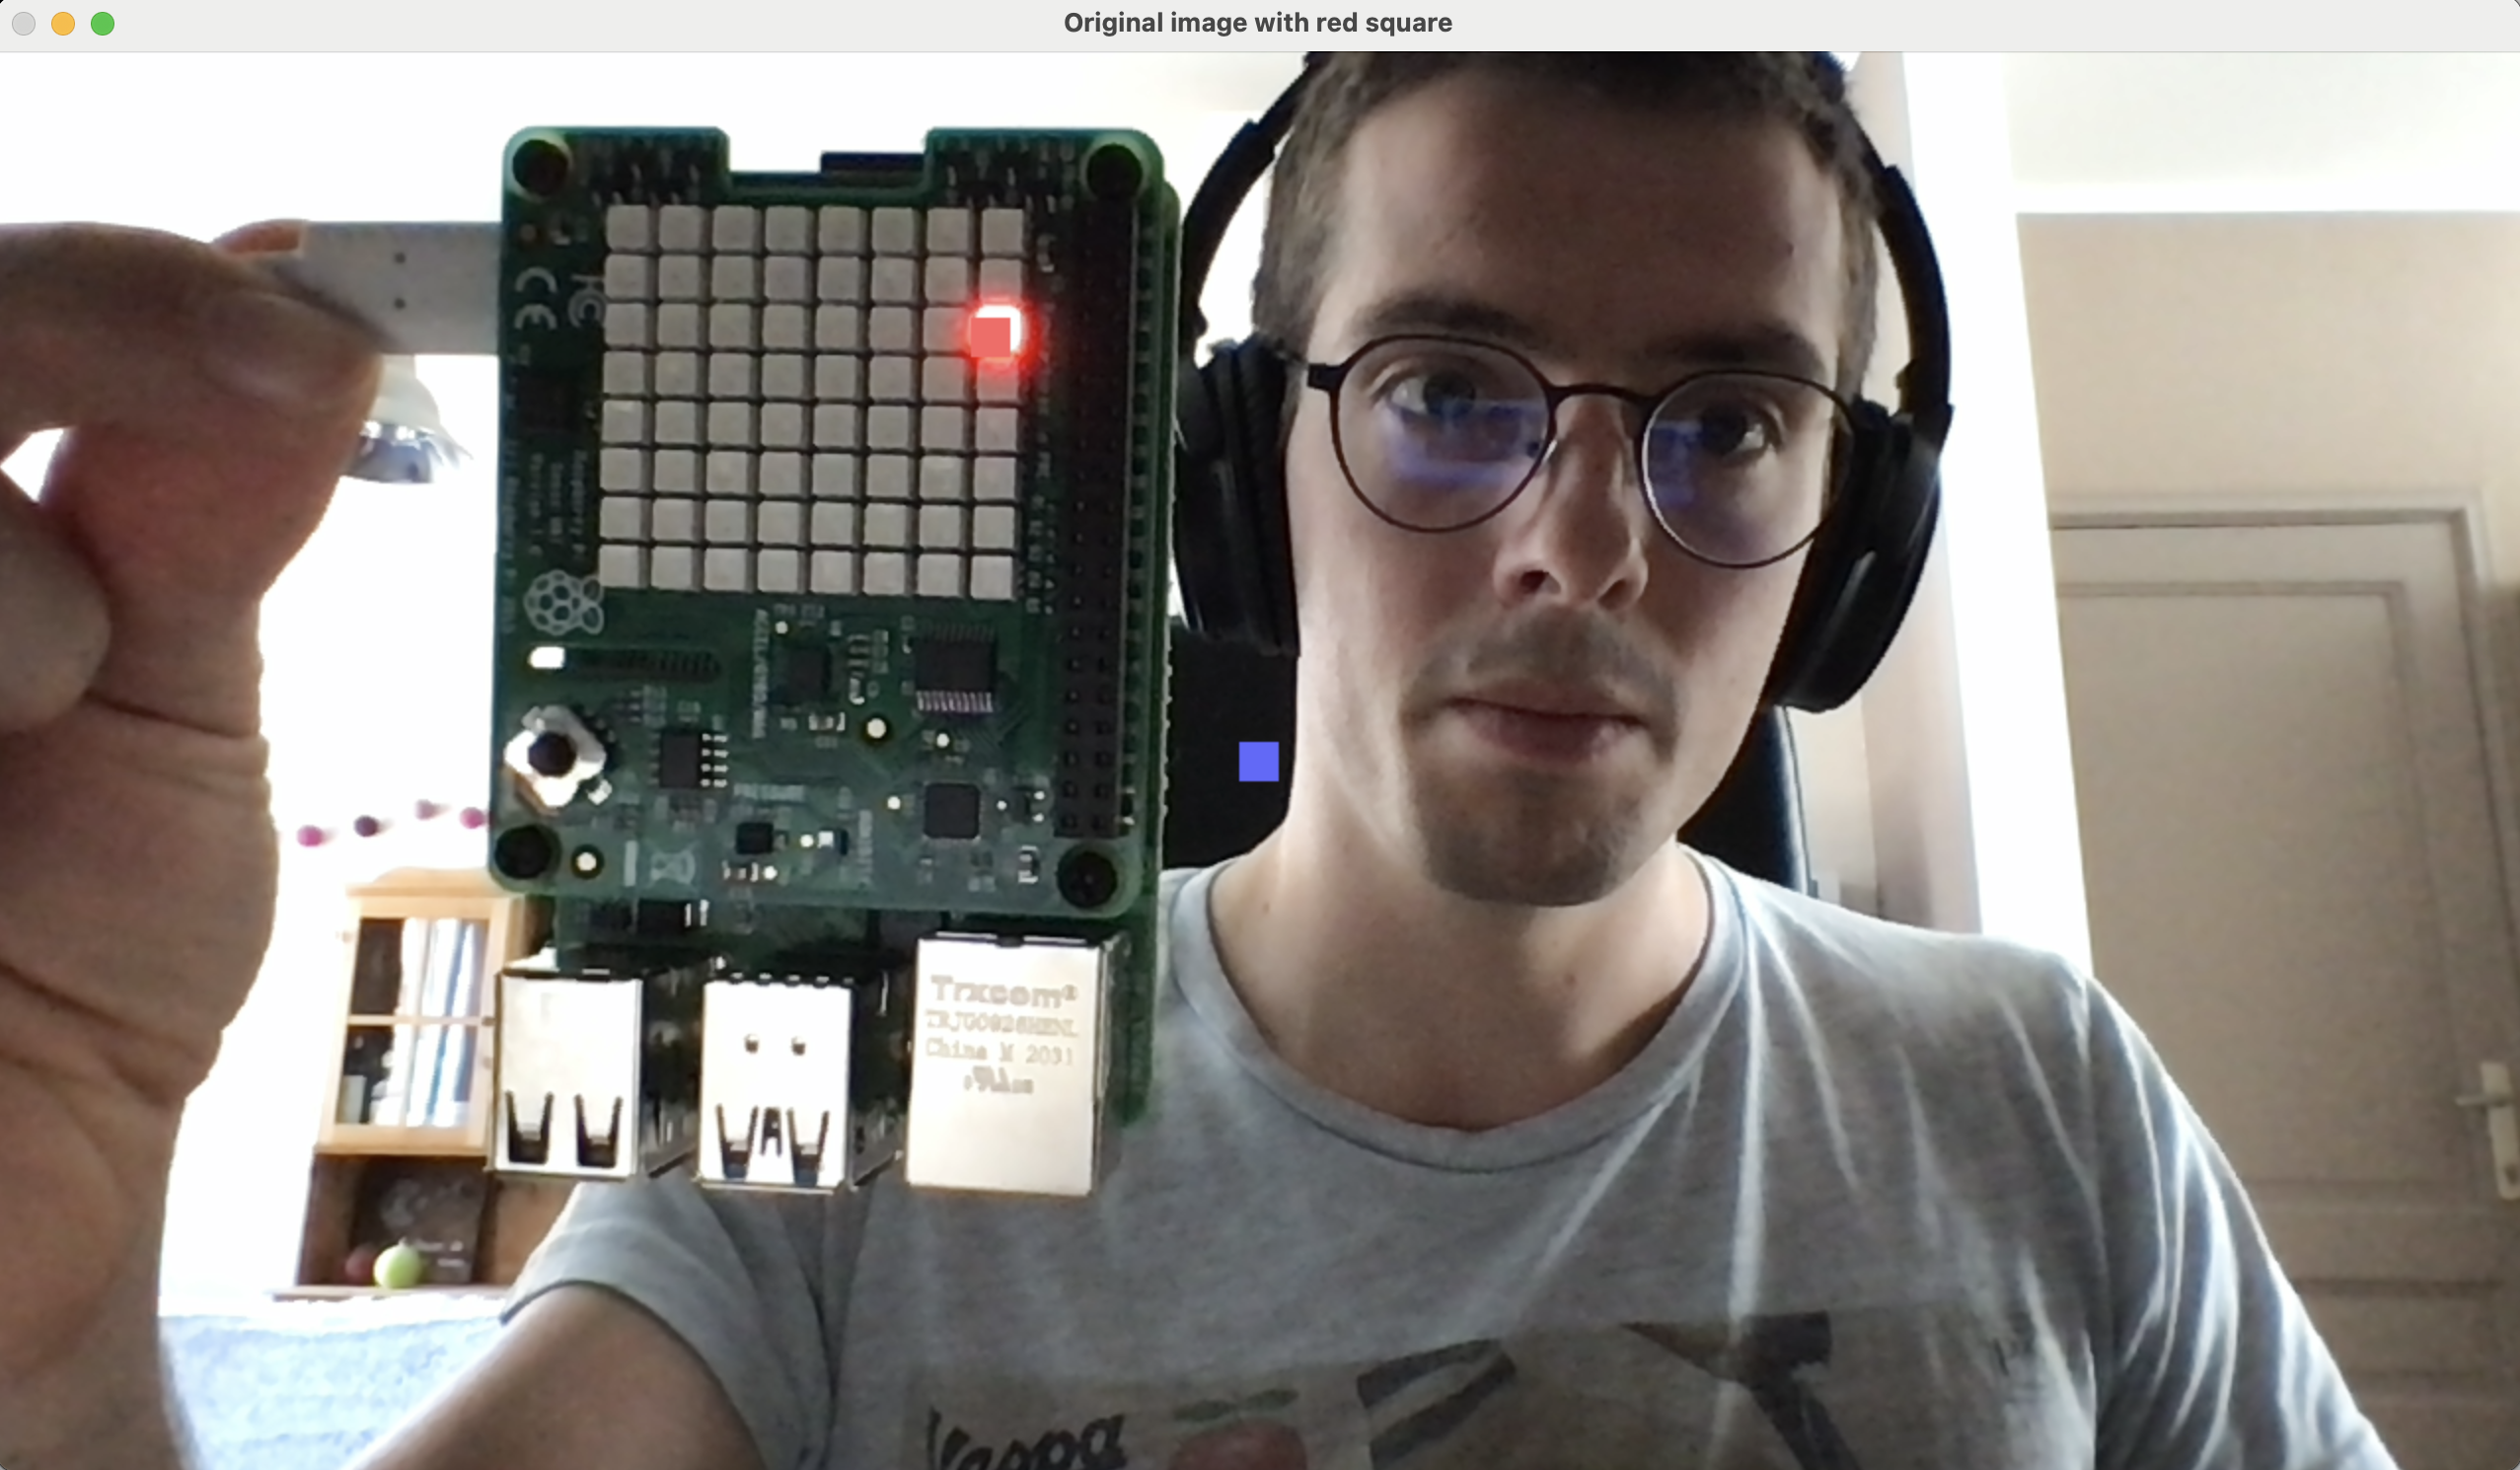
\includegraphics[width=7cm,height=5cm]{Images/original.png}
   \caption{Original webcam image with no filtering.}
   \label{opencv:original}
  \end{minipage}
\hfill
  \begin{minipage}[b]{0.45\linewidth}
   \centering
   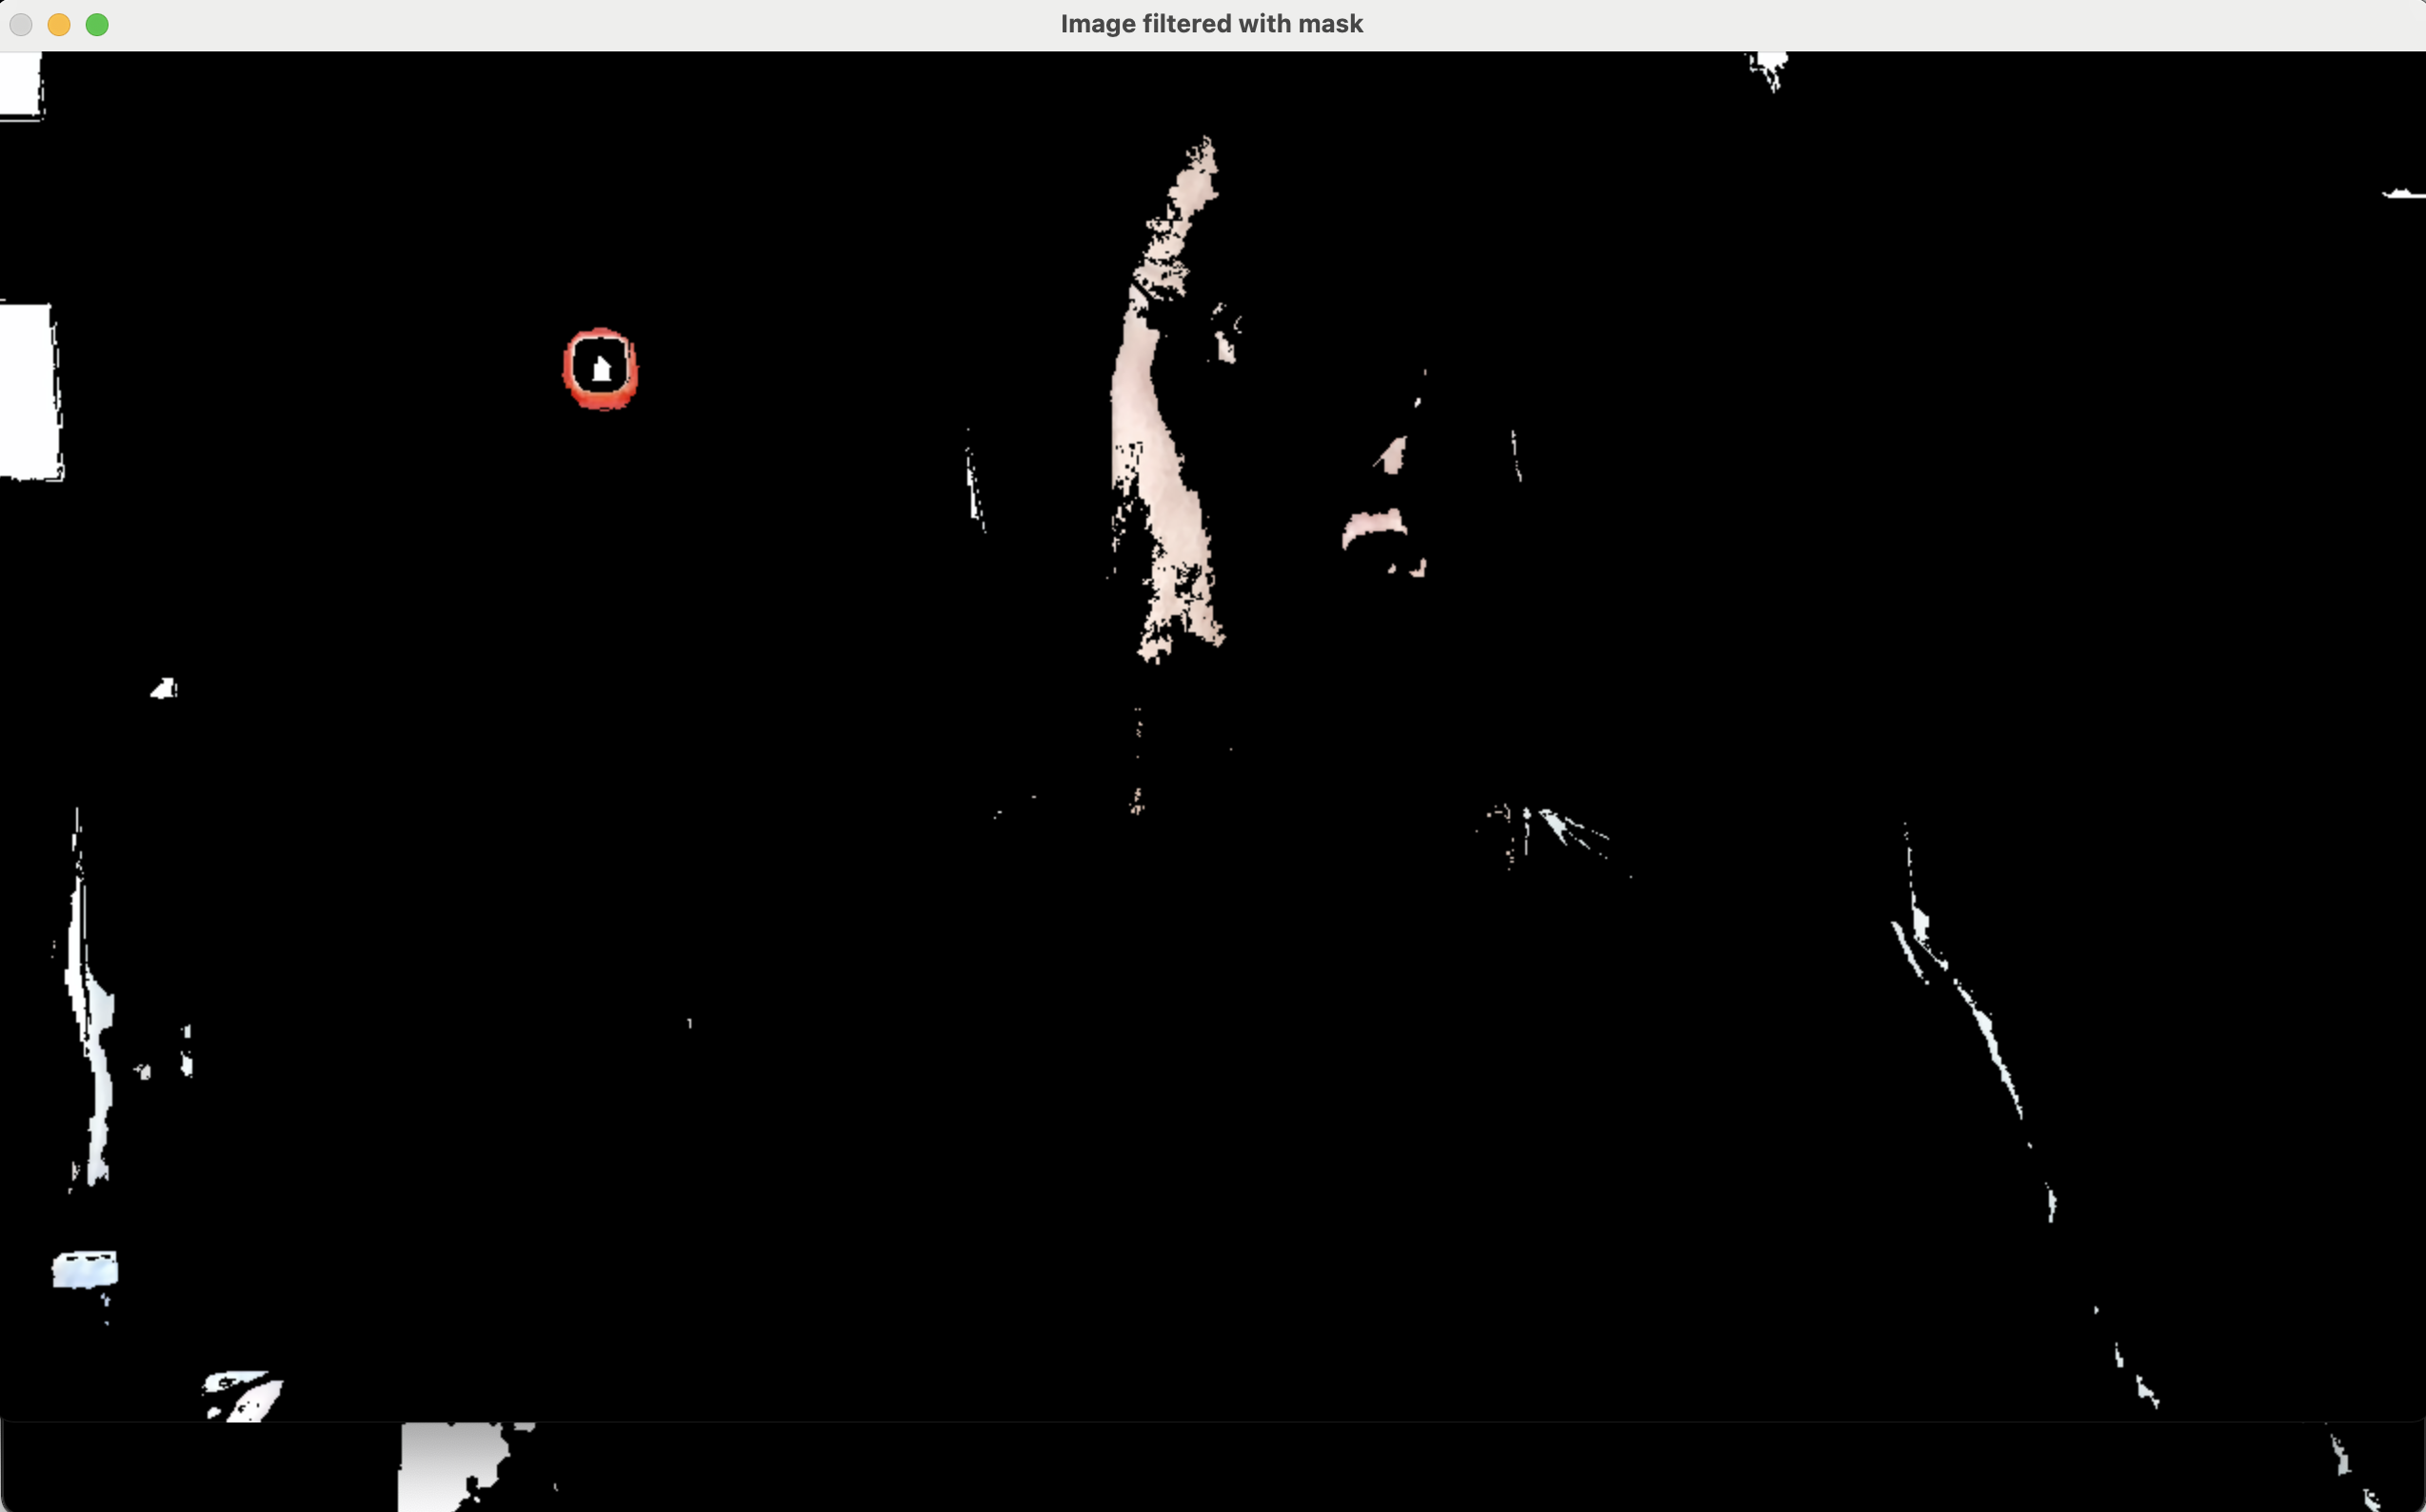
\includegraphics[width=7cm,height=5cm]{Images/red_filter.png}
   \caption{Result of the application of the first red filter.}
   \label{opencv:red_filter}
  \end{minipage}
\end{figure}

\begin{figure}[H]

  \begin{minipage}[b]{0.45\linewidth}
   \centering
   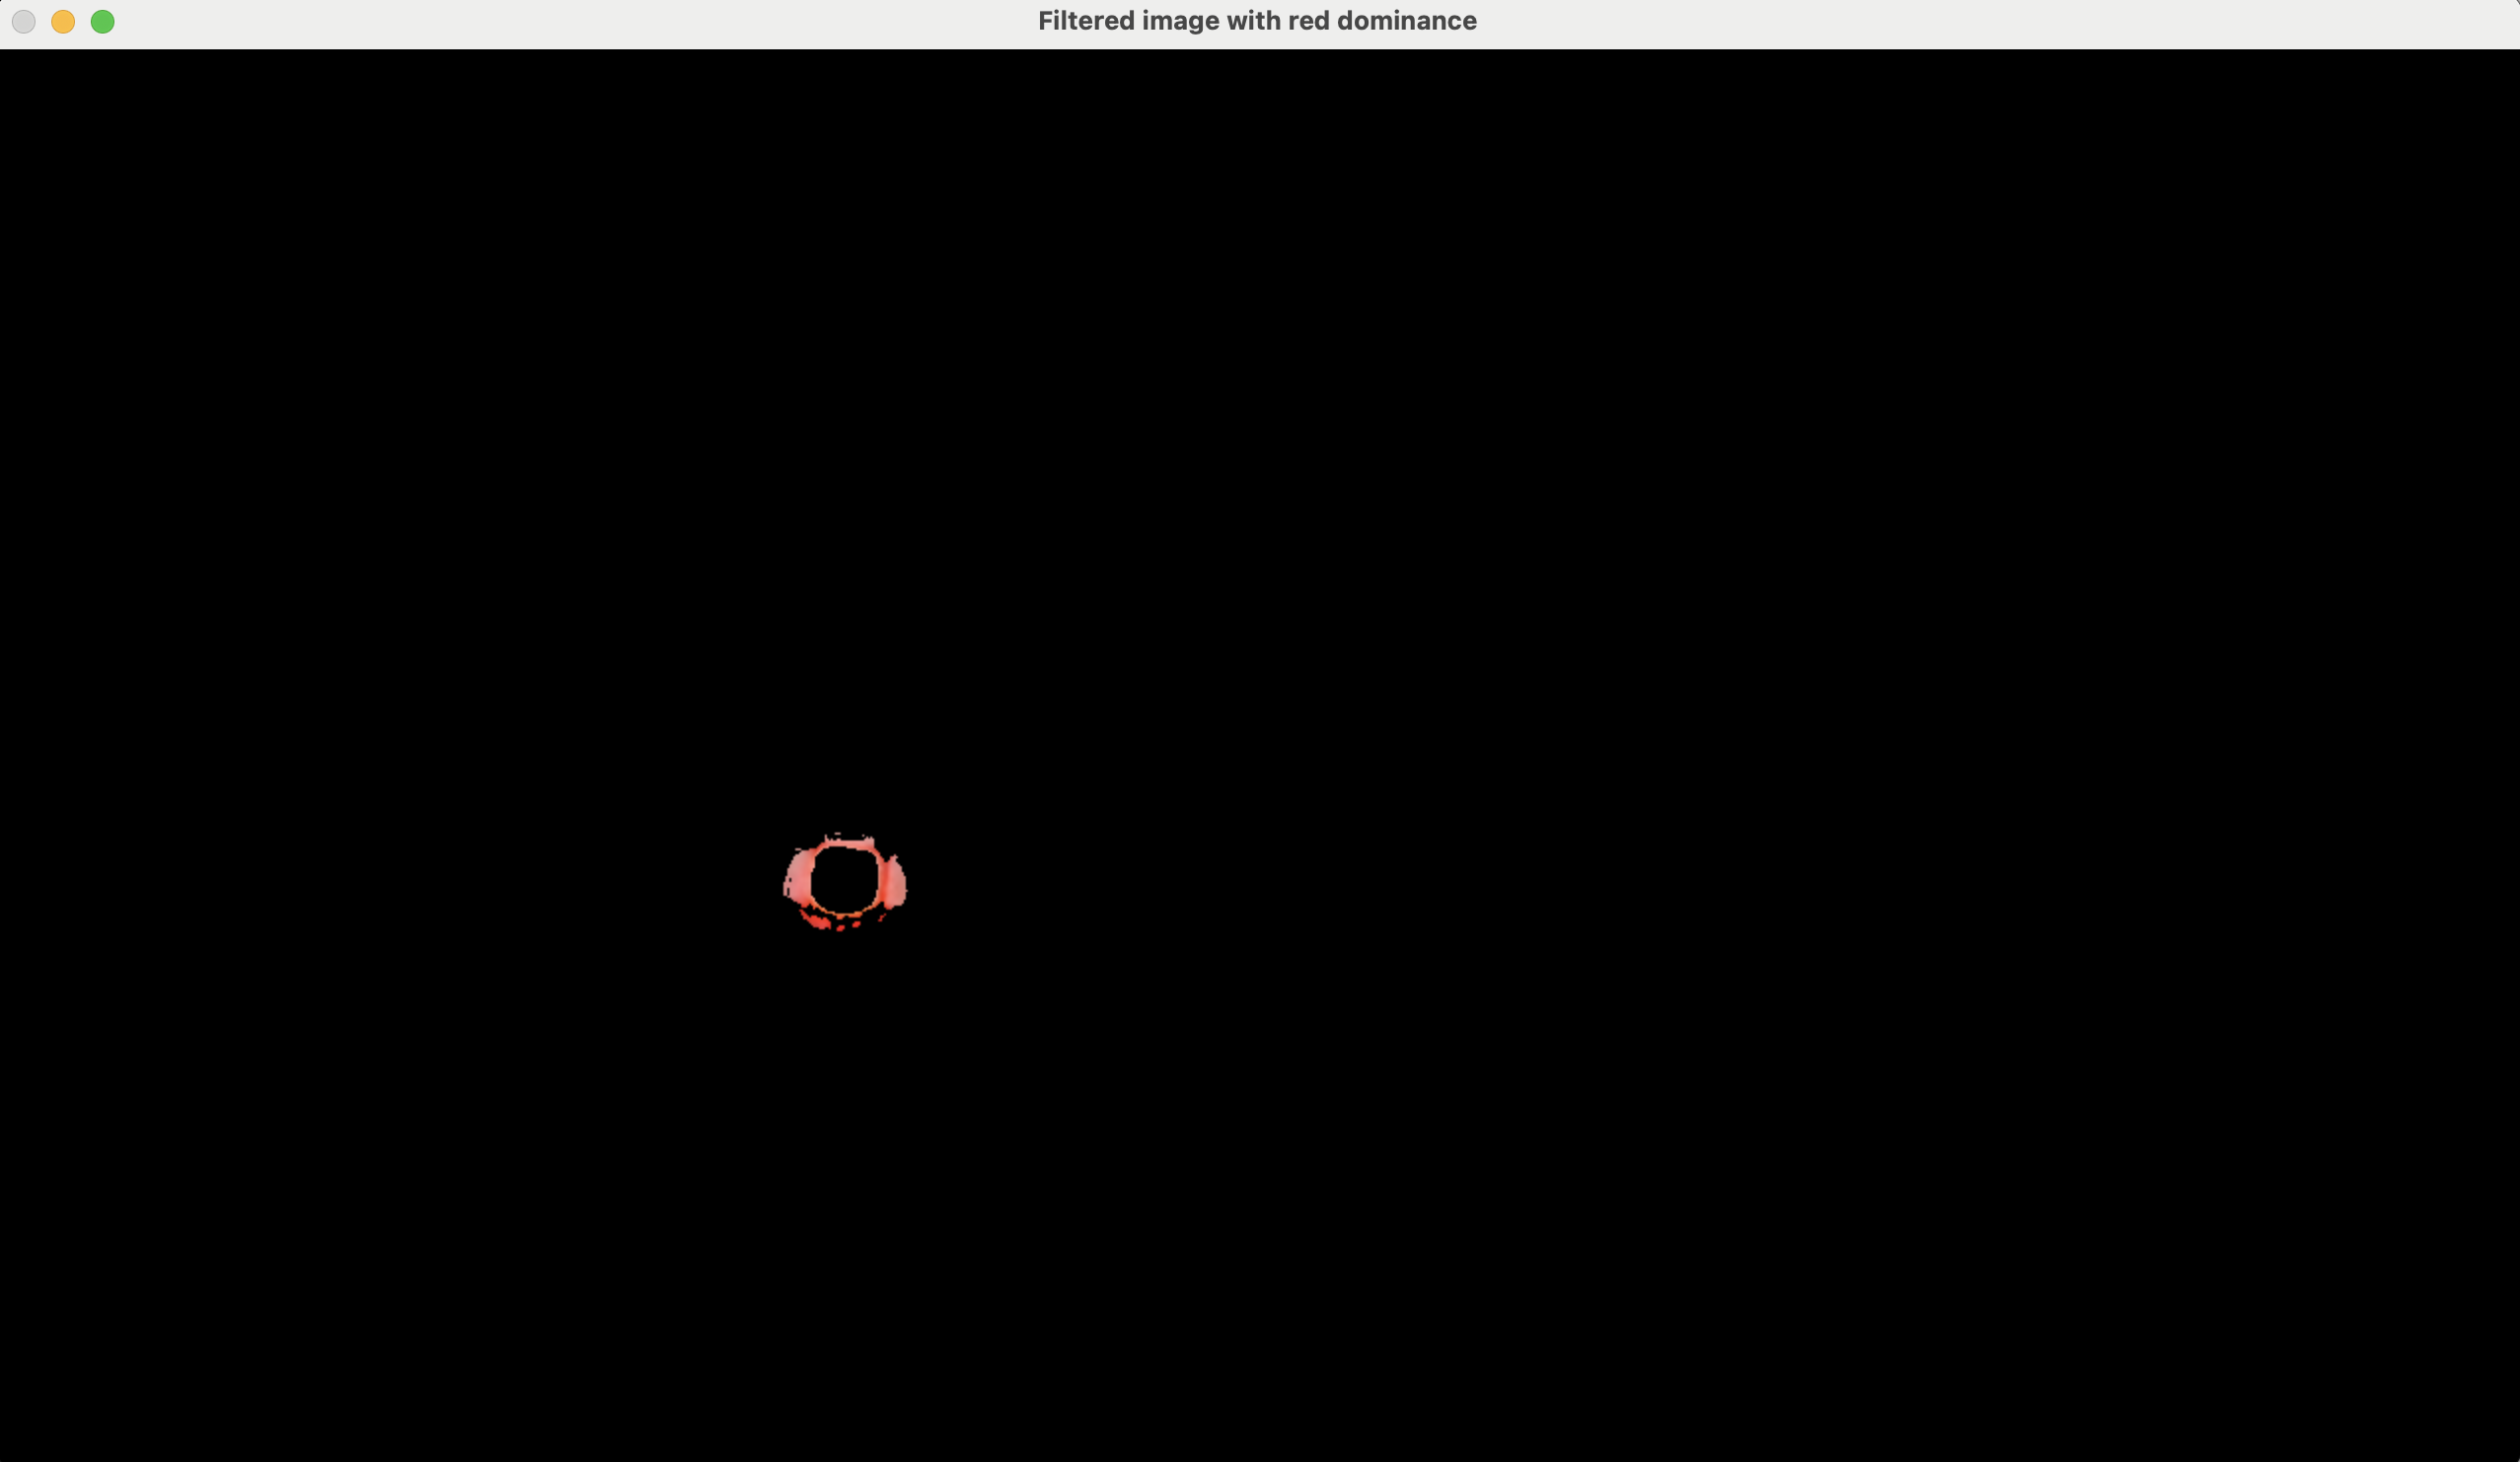
\includegraphics[width=7cm,height=5cm]{Images/additional_red_filter.png}
   \caption{Webcam image after re-applying a red dominance filter on the image of figure \ref{opencv:red_filter}.}
   \label{opencv:add_filter}
  \end{minipage}
\hfill
  \begin{minipage}[b]{0.45\linewidth}
   \centering
   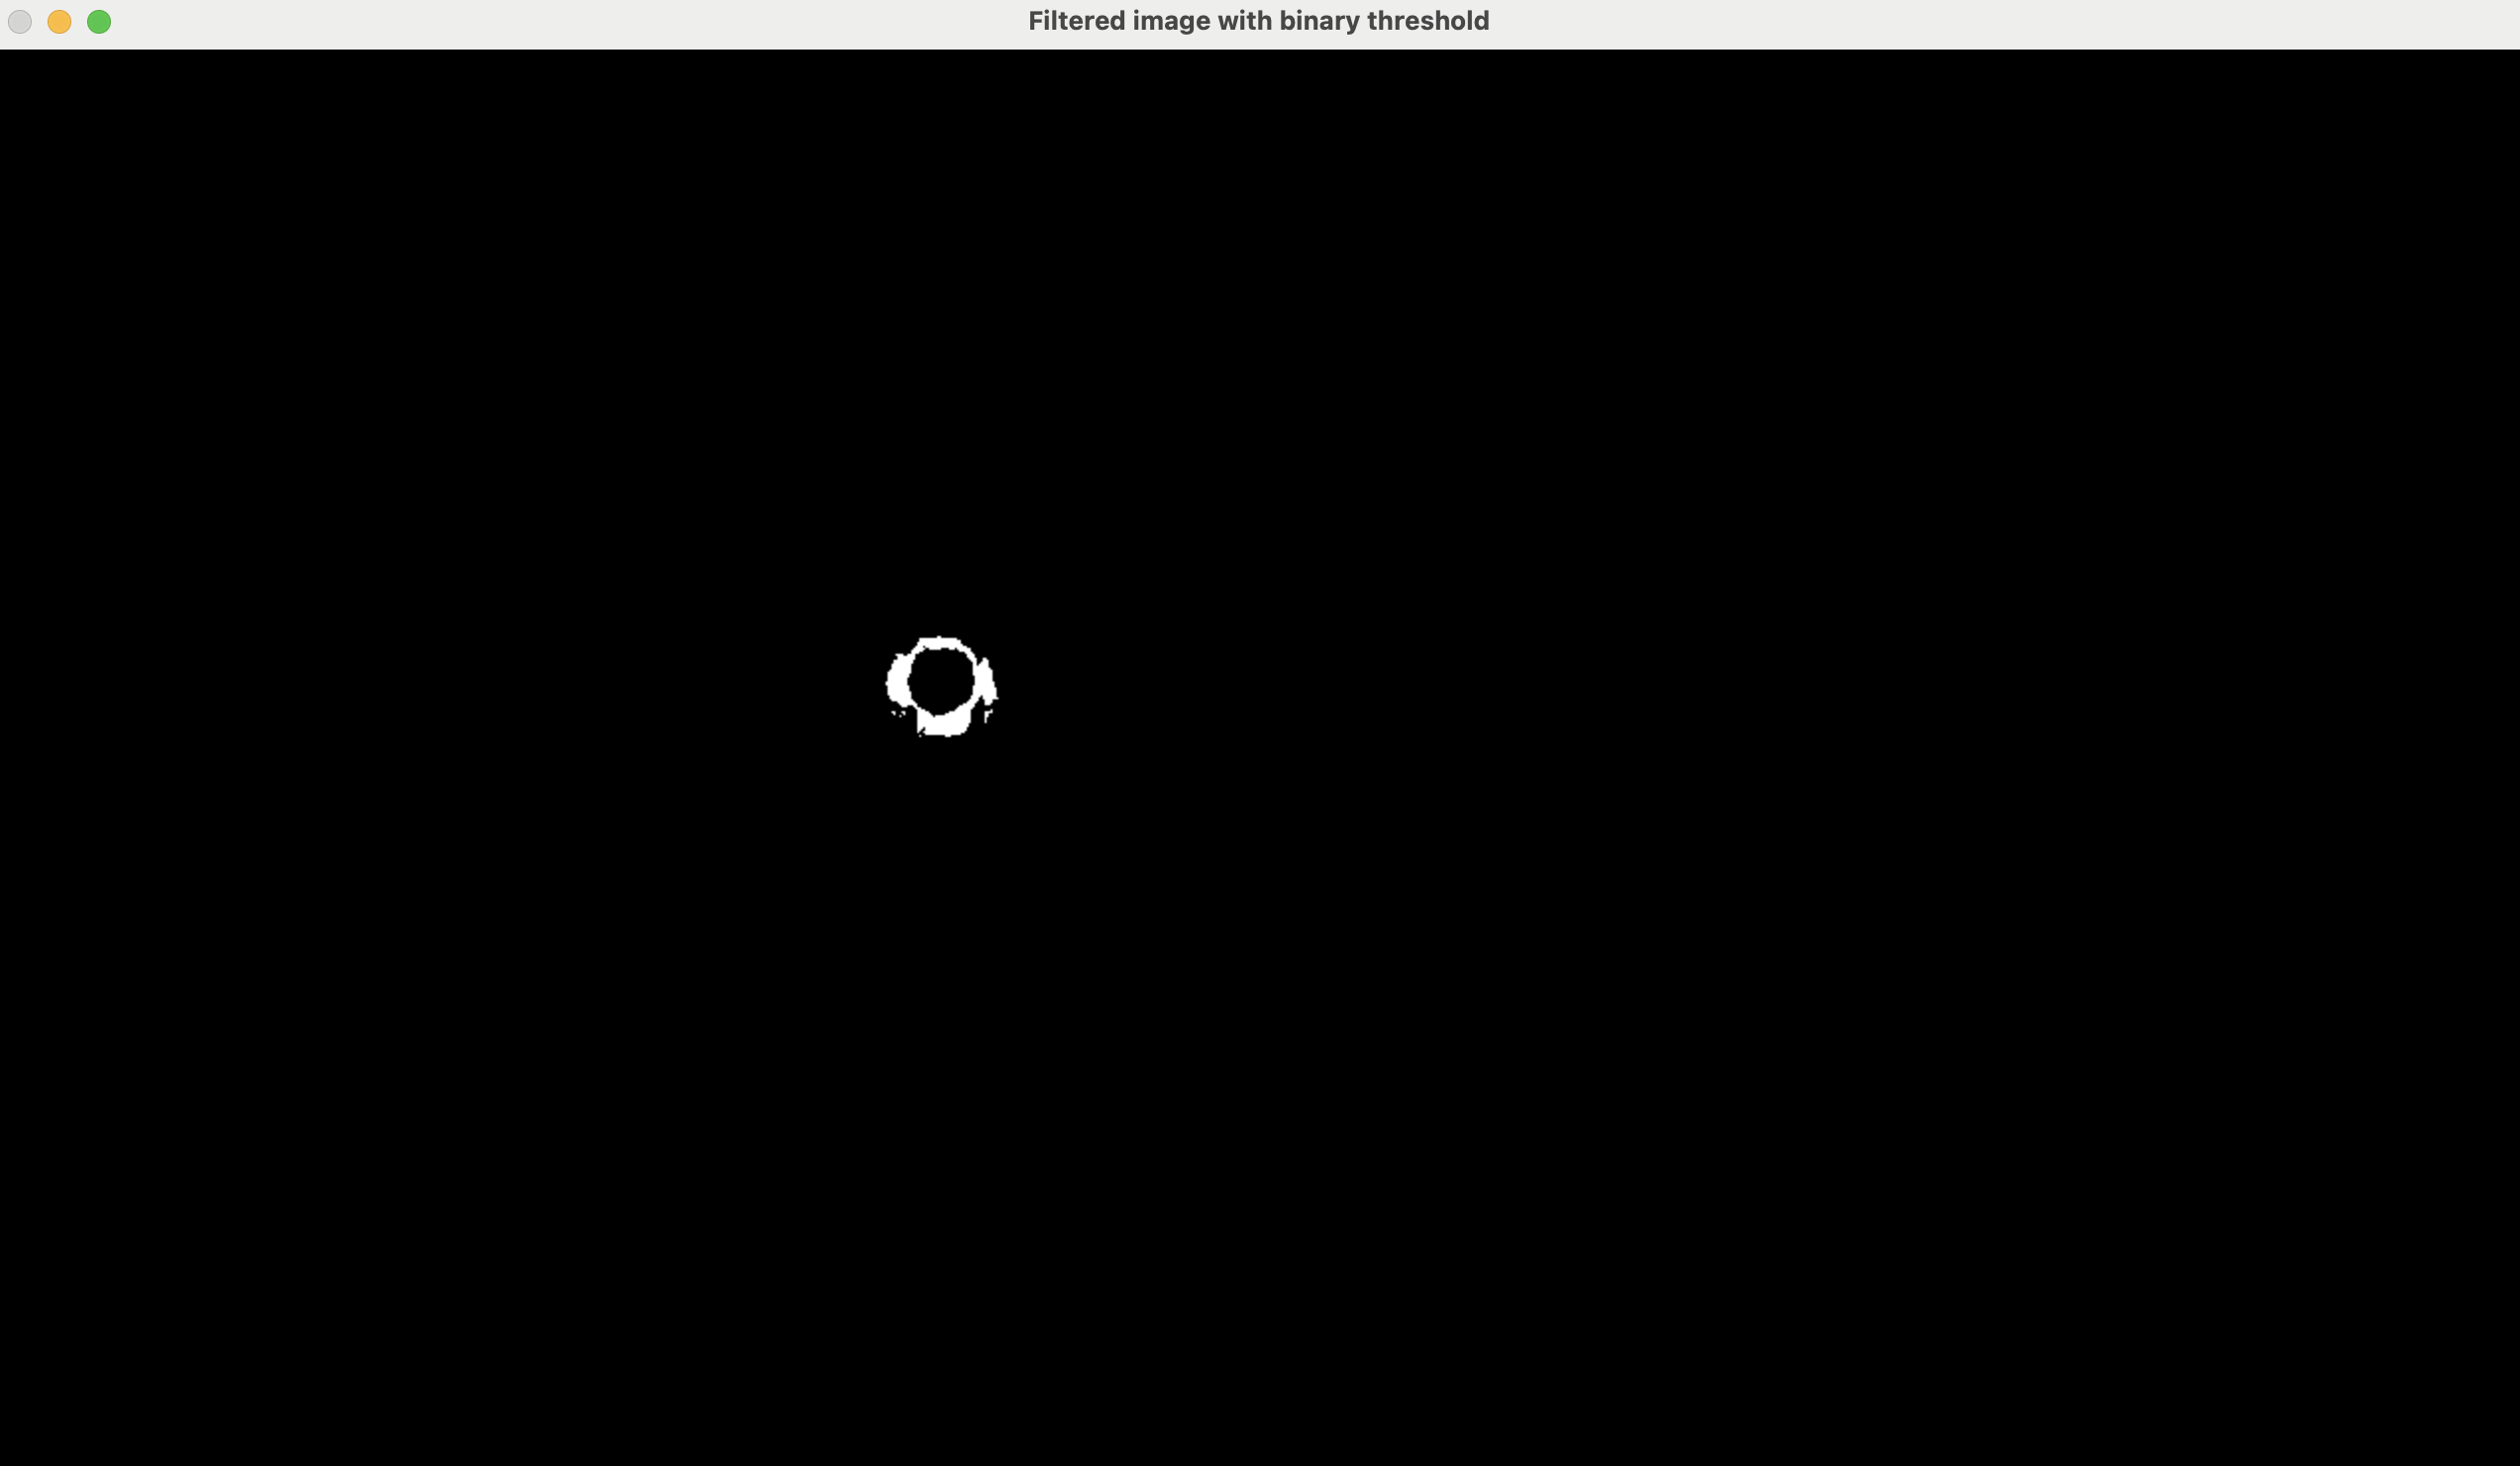
\includegraphics[width=7cm,height=5cm]{Images/threshold.png}
   \caption{Final thresholded image that displays the red dot in gray scale.}
   \label{opencv:threshold}
  \end{minipage}
\end{figure}

Instead of computing the center of a rectangle, it simply computes the center of an arc which gives approximately the same result. Doing so revealed the capturing of the dot's contour to be surprisingly robust against changes in environmental light. The agent therefore benefits from a processing routine \texttt{\detokenize{get_red_dot()}} that allows it to have a reliable access to the red dot's position on the webcam image.

\section{Reinforcement Learning agents}

\chapter{Appendix}

\section{Code on the Raspberry Pi}

\subsection{server.py}
\label{server_code}
\begin{pyverbatim}
import socket
from _thread import *
import pickle
import struct
from sense_hat import SenseHat
from rasp import Raspberry
import time

# Create server
s = socket.socket(socket.AF_INET, socket.SOCK_STREAM)
s.setsockopt(socket.SOL_SOCKET, socket.SO_REUSEADDR, 1)
s.bind(('0.0.0.0', 9395))
s.listen(10)
print("Waiting for a connection")

# Configure Sensehat
sense = SenseHat()
sense.clear()
rasp = Raspberry(sense)

def send(s, data):
    data = pickle.dumps(data)
    s.sendall(struct.pack('>i', len(data)))
    s.sendall(data)

def recv(s):
    data = s.recv(4, socket.MSG_WAITALL)
    data_len = struct.unpack('>i', data)[0]
    data = s.recv(data_len, socket.MSG_WAITALL)
    return pickle.loads(data)

def threaded_client(conn):
    # Declare global variables
    global sense

    while True:
        try:
            data = recv(conn)
            # Place our red dot at desired location
            if isinstance(data, list):
                rasp.place_dot(data)

            # Execute action required by RL agent
            else:
                rasp.move_led(data)

        except:
            pass
        
        # Send Gyroscope and accelerator data
        reply = rasp.acceleration + rasp.orientation
        send(conn, reply)

while True:
    # Accept client
    conn, addr = s.accept()
    print('Connected to:', addr)
    start_new_thread(threaded_client, (conn, ))
\end{pyverbatim}


\subsection{rasp.py}
\label{rasp_code}
\begin{pyverbatim}
import numpy as np


class Raspberry:

    def __init__(self, sense):
        self.sense = sense
        self.acceleration_ = None
        self.orientation_ = None
        self.led = [0, 0]

    @property
    def acceleration(self):
        acc = self.sense.get_accelerometer_raw()
        return [acc['x'], acc['y'], acc['z']]

    @property
    def orientation(self):
        gyro = self.sense.get_gyroscope_raw()
        return [gyro['x'], gyro['y'], gyro['z']]

    def place_dot(self, pos: np.ndarray) -> None:
        self.sense.clear()
        pos = pos[0]
        print("Resettting pixel ({}, {})".format(pos[0], pos[1]))
        self.sense.set_pixel(pos[0], pos[1], (255, 0, 0))

    def move_led(self, action: int) -> None:

        self.sense.clear()
        x, y = self.led[0], self.led[1]

        if action == 0:  # Move to the right
            self.led[0] = x-1 if x>0 else x

        if action == 1:  # Move the the left
            self.led[0] = x+1 if x<7 else x

        if action == 2:  # Move upwards
            self.led[1] = y-1 if y>0 else y

        if action == 3:  # Move down
            self.led[1] = y+1 if y<7 else y
        
        if action == 4:  # Stay at the same position
            self.led[0], self.led[1] = x, y
        
        self.sense.set_pixel(self.led[0], self.led[1], (255, 0, 0))

\end{pyverbatim}

\section{OpenCV code}

\subsection{calibrate.py}
\label{calibrate}

\begin{pyverbatim}
import cv2
import numpy as np


def run():
    while True:

        def nothing(x):
            pass

        # Create a window
        cv2.namedWindow('image')

        # create trackbars for color change
        cv2.createTrackbar('HMin', 'image', 0, 179, nothing)  # Hue is from 0-179 for Opencv
        cv2.createTrackbar('SMin', 'image', 0, 255, nothing)
        cv2.createTrackbar('VMin', 'image', 0, 255, nothing)
        cv2.createTrackbar('HMax', 'image', 0, 179, nothing)
        cv2.createTrackbar('SMax', 'image', 0, 255, nothing)
        cv2.createTrackbar('VMax', 'image', 0, 255, nothing)

        # Set default value for MAX HSV trackbars.
        cv2.setTrackbarPos('HMax', 'image', 179)
        cv2.setTrackbarPos('SMax', 'image', 255)
        cv2.setTrackbarPos('VMax', 'image', 255)

        # Initialize to check if HSV min/max value changes
        hMin = sMin = vMin = hMax = sMax = vMax = 0
        phMin = psMin = pvMin = phMax = psMax = pvMax = 0

        # OpenCV function
        WINDOW_NAME = "Calibration of filter"
        cv2.namedWindow(WINDOW_NAME)  # open a window to show debugging images
        vc = cv2.VideoCapture(0)  # Initialize the default camera

        try:
            if vc.isOpened():  # try to get the first frame
                (readSuccessful, frame) = vc.read()
            else:
                raise (Exception("failed to open camera."))

            while readSuccessful:

                # get current positions of all trackbars
                hMin = cv2.getTrackbarPos('HMin', 'image')
                sMin = cv2.getTrackbarPos('SMin', 'image')
                vMin = cv2.getTrackbarPos('VMin', 'image')

                hMax = cv2.getTrackbarPos('HMax', 'image')
                sMax = cv2.getTrackbarPos('SMax', 'image')
                vMax = cv2.getTrackbarPos('VMax', 'image')

                # Set minimum and max HSV values to display
                lower = np.array([hMin, sMin, vMin])
                upper = np.array([hMax, sMax, vMax])

                # Create HSV Image and threshold into a range.
                hsv = cv2.cvtColor(frame, cv2.COLOR_BGR2HSV)
                mask = cv2.inRange(hsv, lower, upper)
                output = cv2.bitwise_and(frame, frame, mask=mask)

                # Print if there is a change in HSV value
                if ((phMin != hMin) | (psMin != sMin) | (pvMin != vMin) | (phMax != hMax) | (psMax != sMax) | (
                        pvMax != vMax)):
                    print("(hMin = %d , sMin = %d, vMin = %d), (hMax = %d , sMax = %d, vMax = %d)" % (
                        hMin, sMin, vMin, hMax, sMax, vMax))
                    phMin = hMin
                    psMin = sMin
                    pvMin = vMin
                    phMax = hMax
                    psMax = sMax
                    pvMax = vMax

                # Display output image
                cv2.imshow('image', output)
                #############################

                # Set refreshing time
                key = cv2.waitKey(10)
                if key == 27:  # exit on ESC
                    break
                # Get Image from camera
                readSuccessful, frame = vc.read()
        finally:
            vc.release()  # close the camera
            cv2.destroyWindow(WINDOW_NAME)  # close the window


run()

\end{pyverbatim}

\subsection{processing.py}
\label{processing}
\begin{pyverbatim}
import cv2
import numpy as np
from typing import *


def get_red_dot(env, display_images: bool) -> None:

    # Get attributes of environment instance
    frame = env.frame

    # Process the input image from webcam
    total, red, final = filter_image(frame)

    # Place our red dot on image
    x, y, image = compute_red_dot(final, frame)

    if display_images:
        # Display the resulting filtered images
        cv2.imshow('Image filtered with mask', total)
        cv2.imshow('Filtered image with red dominance', red)
        cv2.imshow('Filtered image with binary threshold', final)

    # Display final image with red square on it
    cv2.imshow('Original image with red square', image)

    # Set new square location
    env.square = [x, y]


def filter_image(frame: np.ndarray) -> Tuple[np.ndarray, np.ndarray, np.ndarray]:

    # Convert BGR to HSV format
    _ = cv2.cvtColor(frame, cv2.COLOR_BGR2HSV)

    # lower boundary RED color range values; Hue (0 - 10)
    lower1 = np.array([0, 0, 217])
    upper1 = np.array([10, 255, 255])

    # upper boundary RED color range values; Hue (90 - 180)
    lower2 = np.array([90, 0, 230])
    upper2 = np.array([179, 255, 255])

    # Apply filters defined previously
    lower_mask = cv2.inRange(_, lower1, upper1)
    upper_mask = cv2.inRange(_, lower2, upper2)

    full_mask = lower_mask + upper_mask

    total = cv2.bitwise_and(frame, frame, mask=full_mask)

    # Additional Red color filter
    low_red = np.array([10, 0, 0])
    high_red = np.array([180, 150, 255])
    red_mask = cv2.inRange(total, low_red, high_red)
    red = cv2.bitwise_and(frame, frame, mask=red_mask)

    # Threshold the resulting image
    h, s, v = cv2.split(red)
    ret, final = cv2.threshold(v, 150, 255, cv2.THRESH_BINARY)

    return total, red, final


def compute_red_dot(final: np.ndarray, frame: np.ndarray) -> Tuple[Union[None, float], Union[None, float], np.ndarray]:

    # Dilatation of filtered image
    dilatation = cv2.dilate(final, np.ones((3, 3)))
    retval, labels, stats, centroids = cv2.connectedComponentsWithStats(dilatation)

    # Compute position of biggest red area
    x, y = None, None
    max_area = None

    for stat, center in zip(stats[1:], centroids[1:]):
        area = stat[4]

        if (max_area is None) or (area > max_area):
            x, y = center
            max_area = area

    image = np.copy(frame)

    # Put blue square at the center of the image
    image[360 - 10:360 + 10, 640 - 10:640 + 10, :] = (255, 100, 100)

    if x is not None and y is not None:
        x, y = int(x), int(y)
        image[y - 10:y + 10, x - 10:x + 10, :] = (100, 100, 255)
        return float(x), float(y), image

    else:
        return x, y, image

\end{pyverbatim}


